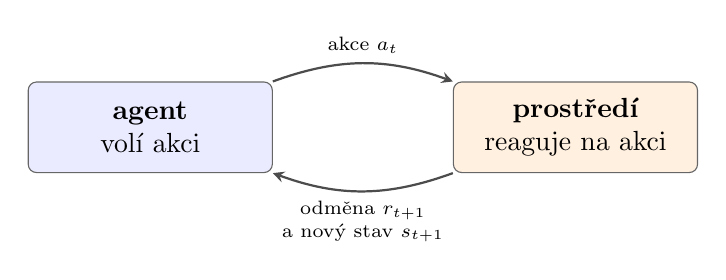
\begin{tikzpicture}[
    >=stealth,
    box/.style={
        draw=black!60,
        rounded corners=3pt,
        minimum width=3.1cm,
        minimum height=1.15cm,
        align=center
    },
    arr/.style={
        ->,
        thick,
        draw=black!70
    }
]

    \node[
        box,
        fill=blue!8
    ] (agent) at (-2.7,0)
        {\textbf{agent}\\
         volí akci};

    \node[
        box,
        fill=orange!12
    ] (environment) at (2.7,0)
        {\textbf{prostředí}\\
         reaguje na akci};

    \draw[arr]
        (agent.north east)
        to[bend left=20]
        node[
            above,
            font=\scriptsize
        ] {akce $a_t$}
        (environment.north west);

    \draw[arr]
        (environment.south west)
        to[bend left=20]
        node[
            below,
            align=center,
            font=\scriptsize
        ] {odměna $r_{t+1}$\\a nový stav $s_{t+1}$}
        (agent.south east);

\end{tikzpicture}
